\documentclass[a4paper,12pt,french]{article}

\usepackage[TD]{../../../Style}

\renewcommand\tabularxcolumn[1]{m{#1}}

\geometry{left=13mm, right=13mm, top=10mm, bottom=17mm, marginparwidth=15mm}

\setlist[itemize]{align=parleft,left=5pt..15pt}
\setlist[enumerate]{align=parleft,left=5pt..20pt}

\setlength\columnsep{20pt}

%Sources: Indice 1Tech, Hyperbole 2nde, Indice 2nde (2019), perso, fiche Thomas

% Début du document
%%%%%%%%%%%%%%%%%%%
\begin{document}

\titre{Proportions, variations - Exercices}

\begin{multicols*}{2}

\section{Proportions}

\begin{exercice}
Parmi les 200 spectateurs d'une salle de cinéma, 64 ont bénéficié d'un tarif réduit. Calculer le pourcentage de spectateurs ayant bénéficié d'un tarif réduit.
\end{exercice}

\begin{exercice}
On considère le tableau suivant qui donne la répartition des salariés d'une start-up.
\begin{center}
\begin{tabularx}{\linewidth}{
|>{\centering\arraybackslash}c
|>{\centering\arraybackslash}X
|>{\centering\arraybackslash}X
|>{\centering\arraybackslash}X|} \cline{2-4} \multicolumn{1}{c|}{}
& Hommes & Femmes & Total \\ \hline
Commerciaux & 15 & 9 & 24 \\ \hline
Développeurs & 7 & 9 & 16 \\ \hline
Total & 22 & 18 & 40 \\ \hline
\end{tabularx}
\end{center}
Calculer:
\begin{enumerate}
\item La proportion de femmes dans cette startup.
\item Celle des hommes développeurs parmi les développeurs.
\item Celle des femmes parmi les commerciaux?
\item Celle des commerciales parmi les femmes?
\end{enumerate}
\end{exercice}

\begin{exercice}
Il y a $34$ élèves en \seconde 12, dont 18 filles. Calculer la proportion de filles dans la classe, arrondie au pourcent près.
\end{exercice}

\begin{exercice}
$25 \%$ des 1800 élèves d'un lycée sont en seconde. Combien cela représente-t-il d'élèves?
\end{exercice}

\begin{exercice}
Sur l'étiquette d'une bouteille de jus multifruits, on lit: "$70 \%$ de jus d'agrumes, dont $30 \%$ de jus de mandarine". Quel est le pourcentage de jus de mandarine dans cette boisson?
\end{exercice}

\begin{exercice}
La moitié de la carte d'un restaurant est composée de plats végétariens. Parmi ceux-ci, 20 $\%$ contiennent des tomates. Déterminer la proportion de plats végétariens contenant des tomates dans la carte du restaurant.
\end{exercice}

\section{Variations absolues, relatives}

\begin{exercice}
Un appartement était loué à $400$\euro{} par mois. Suite à un changement de locataire, le loyer s'élève maintenant à $440$\euro . De quel pourcentage a augmenté le loyer de cet appartement?
\end{exercice}

\begin{exercice}
Le tableau suivant donne le PIB du Brésil et des Etats-Unis en 2000 et en 2010 (en milliards de dollars):
\begin{center}
\begin{tabularx}{0.9\linewidth}{
|>{\centering\arraybackslash}c
|>{\centering\arraybackslash}X
|>{\centering\arraybackslash}X|} \cline{2-3} \multicolumn{1}{c|}{}
& 2000 & 2010 \\ \hline
Brésil & 655 & 2209 \\ \hline
Etats-unis & 10285 & 14964 \\ \hline
\end{tabularx}
\end{center}
\begin{enumerate}
\item Déterminer la variation absolue du PIB entre 2000 et 2010 pour chacun de ces pays.
\item Déterminer leur évolution relative.
\end{enumerate}
\end{exercice}

\begin{exercice}
Le diagramme ci-dessous indique le nombre d'utilisateurs de réseaux sociaux dans le monde en 2016, 2017 et 2018:
\begin{centrer}
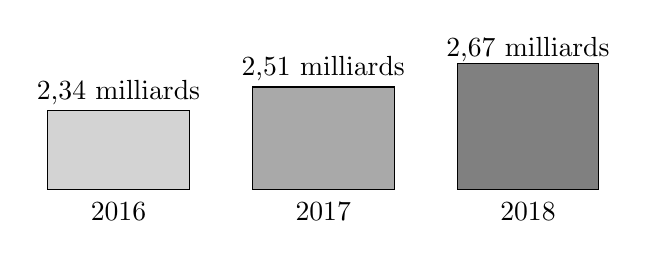
\begin{tikzpicture}
\draw[fill=LightGray] (0,0) rectangle (1.8,1) node[midway,below=5.5mm]{2016} node[midway,above=4.5mm]{2,34 milliards};
\draw[fill=DarkGray] (2.6,0) rectangle (4.4,1.3) node[midway,below=7mm]{2017} node[midway,above=6mm]{2,51 milliards};
\draw[fill=Gray] (5.2,0) rectangle (7,1.6) node[midway,below=8.5mm]{2018} node[midway,above=7mm]{2,67 milliards};
\end{tikzpicture}
\end{centrer}
\noindent Calculer la variation absolue, puis relative de 2016 à 2017, puis de 2017 à 2018.
\end{exercice}

\begin{exercice}
Un théâtre a programmé 260 représentations pour l'année en cours contre 240 l'année passée. Calculer le taux d'évolution du nombre de représentations entre l'année passée et l'année en cours.
\end{exercice}

\begin{exercice}
En septembre 2000, la superficie minimum de la banquise arctique était de $6,32$ millions de km$^2$. Elle n'était plus que de $4,59$ millions de km$^2$ en septembre 2018. De quel pourcentage la superficie de la banquise arctique a-t-elle diminué entre septembre 2000 et septembre 2018?
\end{exercice}

\section{Taux d'évolution et CM}

\begin{exercice}
Compléter:
\begin{enumerate}
\item Augmenter une quantité de $40 \%$ revient à la multiplier par \ldots
\item Diminuer une quantité de $30 \%$ revient à la multiplier par \ldots
\end{enumerate}
\end{exercice}

\begin{exercice} \

\begin{enumerate}
\item Donner le coefficient multiplicateur correspondant aux taux d'évolution suivants:
\end{enumerate}
\begin{tabularx}{1.05\linewidth}{XXXX}
\fakeitem $+0,1$ & \fakeitem $+200 \%$ & \fakeitem $-50 \%$ & \fakeitem $-0,7$
\end{tabularx}
\begin{enumerate}[resume]
\item Donner le pourcentage d'évolution correspondant aux coefficients multiplicateurs suivants:
\end{enumerate}
\begin{tabularx}{1.05\linewidth}{XXXX}
\fakeitem $2$ & \fakeitem $0,75$ & \fakeitem $1,04$ & \fakeitem $0,37$
\end{tabularx}
\end{exercice}

\begin{exercice}
Vrai ou faux?
\begin{enumerate}
\item Multiplier par 0,6, c'est diminuer de $40 \%$.
\item Un livre ancien coûte $68$ \euro . Après une hausse de $127 \%$, son prix est $35,27$ \euro .
\end{enumerate}
\end{exercice}

\begin{exercice}
Un adolescent mesure $1,60$m lors de son arrivée au lycée. Au cours de l'année de Seconde, sa taille augmente de $5 \%$. Quelle est sa taille à la fin de l'année?
\end{exercice}

\begin{exercice}
Pendant les vacances, Léa passe deux heures par jour sur sa console. Ses parents lui ont demandé de réduire ce temps de $80 \%$ lorsque les cours reprendront. Combien de temps pourra-t-elle espérer jouer après la rentrée?
\end{exercice}

\begin{exercice}
Une boulangerie propose une baguette de pain à $90$ centimes. Son prix augmente de $10 \%$. Par quel nombre a-t-il été multiplié? Quel est alors son nouveau prix?
\end{exercice}

\begin{exercice}
En France, le taux de TVA est $20 \%$. Un industriel fournit des radiateurs à un grossiste à un prix unitaire de $84$\euro{} hors taxes. Quel est le prix TTC d'un matelas?
\end{exercice}

\begin{exercice}
Un hôpital a une capacité de $110$ lits. En janvier, 60 lits sont occupés par des mineurs tandis qu'en février, le nombre de lits occupés par des majeurs a augmenté de $20 \%$. Combien de lits sont occupés par des majeurs en février?
\end{exercice}

\section{Evolutions réciproques}

\begin{exercice}
Vrai ou faux? Un prix augmente de $20 \%$ puis diminue de $20 \%$. Il est donc revenu à sa valeur initiale.
\end{exercice}

\begin{exercice}
Après une augmentation de $10 \%$, un produit coûte $110$\euro{}. Quel était son prix initial?
\end{exercice}

\begin{exercice}
Compléter le schéma suivant: \vspace{1mm}
\begin{centrer}
\begin{tikzpicture}
\node[draw,ellipse,thick,minimum height=1cm,minimum width=2cm] (V0) at (0,0) {$1500$};
\node[draw,ellipse,thick,minimum height=1cm,minimum width=2cm] (V1) at (6,0) {};
\draw[->,>=latex,thick] (V0) to[bend left=20] node[midway,above=5pt]{$\times \ldots$} node[midway,below]{$+ 26 \%$} (V1);
\draw[->,>=latex,thick] (V1) to[bend left=20] node[midway,below=5pt]{$\times \ldots$} node[midway,above]{\makebox[2cm]{\dotfill}} (V0);
\end{tikzpicture}
\end{centrer}
\end{exercice}

\begin{exercice}
Vrai ou faux?
\begin{enumerate}
\item Après une diminution de $12 \%$, on obtient 100. Alors la valeur initiale était 112.
\item Après une augmentation de $22 \%$, on obtient 122. Alors la valeur initiale était 100.
\end{enumerate}
\end{exercice}

\section{Evolutions successives}

\begin{exercice}
Le prix d'un litre d'essence a augmenté de $15 \%$ entre janvier et juillet, puis de $10 \%$ entre juillet et décembre.
\begin{enumerate}
\item Calculer le coefficient multiplicateur de ces deux évolutions.
\item Justifier que le coefficient multiplicateur global est $1,265$.
\end{enumerate}
\end{exercice}

\begin{exercice}
La première semaine des soldes, un magasin propose $40 \%$ de réduction sur tous les vêtements. Lors de la deuxième démarque, le magasin accorde $20 \%$ de remise supplémentaire.
\begin{enumerate}
\item Calculer le coefficient multiplicateur de ces deux évolutions.
\item En déduire le coefficient multiplicateur global, puis le taux d'évolution global des prix.
\end{enumerate}
\end{exercice}

\begin{exercice}
Une commune organise chaque année une course à pied dans les rues de son centre. En 2017, le nombre de participants a augmenté de $20 \%$ mais en 2018, il a baissé de $12 \%$. Quel est le taux d'évolution du nombre de coureurs sur ces deux années?
\end{exercice}

\begin{exercice}
Une oeuvre d'art est achetée par Karim. Il la revend à Clara en faisant une plus-value de $35 \%$. Clara la revend à son tour à Nicolas en faisant un bénéfice de $16 \%$. Sachant que Nicolas a acheté cette oeuvre $70470$\euro{}, combien Karim l'a-t-il achetée au départ?
\end{exercice}

\Centering\rule{0.8\linewidth}{1pt}

\begin{exercice}
Voici trois situations et trois calculs. Associer chaque situation à un calcul en imaginant une question.
\begin{enumerate}
\item Un ordinateur coute $450$\euro{}. Un commerçant accorde une remise de $6\%$.
\item La longueur d'une piste d'ULM est $450$m. On l'augmente de $6 \%$.
\item $6 \%$ des 450 pompiers d'une ville ont moins de 20 ans.
\end{enumerate}

\noindent A. $450 \times 1,06$ \hfill B. $450 \times 0,06$ \hfill C. $450 \times 0,94$
\end{exercice}

\begin{exercice}
Un pull rétrécit de $1 \%$ à chaque séchage en machine. Après trois séchages, la longueur des manches est $59.4$ cm. Quelle était cette longueur, en cm, avant les trois séchages? On arrondira au dixième près.
\end{exercice}

\begin{exercice}
Alexis a placé une somme d'argent au taux de $1.75 \%$, les intérêts étant calculés annuellement et ajoutés au solde du compte. Il affirme: "Si je n'effectue aucun retrait et si le taux ne change pas, le solde de mon compte aura plus que doublé dans 40 ans!"
A-t-il raison? Expliquer.
\end{exercice}

\end{multicols*}

\end{document}
